\chapter{Preparation}

{\sf \color{red}
  Principally, this chapter should \textbf{describe the work which was
  undertaken before code was written}, hardware built or theories worked on. It
  should \textbf{show how the project proposal was further refined and
  clarified}, so that the Implementation stage could go smoothly rather than by
  trial and error.

  Throughout this chapter and indeed the whole dissertation, it is essential to
  \textbf{demonstrate that a proper professional approach was employed}.

  The nature of this chapter will vary greatly from one dissertation to another
  but, underlining the professional approach, this chapter will very likely
  include a \textbf{section headed “Requirements Analysis”} and
  \textbf{incorporate other references to the techniques of Software
  Engineering}.

  The chapter will cite any \textbf{new programming languages and systems which
  had to be learnt} and will \textbf{mention complicated theories or
algorithms} which required understanding.

  It is essential to \textbf{declare the Starting Point} (see Section 7). This
  states \textbf{any existing codebase or materials} that your project builds
  on.  The text here \textbf{can commonly be identical to the text in your
  proposal}, but it may \textbf{enlarge on it or report variations}. For
  instance, the true starting point may have turned out to be different from
  that declared in the proposal and \textbf{such discrepancies must be
  explained}.
}

Before commencing implementation of the project, careful consideration was
given to planning it. Current solutions were explored, studied and evaluated
against the aims described in Section~\ref{intro:aims}. The rest of this
chapter will explain the initial set-up, elaborate on findings concerning
related work and outline the project's starting point.

\section{Project Planning}

This project presents a unique idea and breaks new ground. As such, the
methodology had to suit and reflect the largely exploratory nature of the
process. A spiral software development model was chosen: think of an idea,
modify the model (of Coq proof-objects), implement and propogate the necessary
changes, evaluate the end-result and repeat. This allowed for experimentation
of ideas and flexibility of implementation strategies.

Git (\href{http://git-scm.com}{\texttt{git-scm.com}}) and GitHub
(\href{http://github.com/dc-mak}{\texttt{github.com/dc-mak}}) were invaluable during the
project, allowing for easy tracking, reverting, reviewing and collaborating.
New features could be tested on new branches before being merged in and a copy
of the work was safely backed up in one more place. GitHub extensions such as
Travis-CI (continous integration) were added in later, as it became apparent
that precisely specified versioning, build-dependencies and automated tests were
useful in spotting errors early.

\section{Requirements Analysis}
Several components of this project needed to function correctly, both
individially and in conjuction for it to work. Separate parts for
modelling/translation (from Coq to the chosen model), displaying and
interacting (Neo4j/Cypher) and computation (Neo4j/Cypher plugins)
needed to be developed and brought together. Below is a list of required
features used throughout development to guide and provide context for
implementation decisions.

\begin{itemize}

  \item \textbf{Modelling}: The model should
  \begin{itemize}

    \item include as much relevant data as possible. Here, relevant means
          useful to understanding a large library, but not so much so as to
          obfuscate any information or make learning how to use the project
          more difficult.

    \item be flexible to work with and easy to translate. One could imagine
          different front-ends for interacting with and computing data
          from the model.

    \item strike a balance between size and precomputing too much data.
          Figuring out which pieces of data can be reconstructed later and
          which are beneficial to compute during modelling will be a matter of
          experimentation and weighing up ease of implementation
          versus ease of later processing.

  \end{itemize}

  \item \textbf{Interaction}: Interacting with the model should
  \begin{itemize}

    \item primarily, allow users to understand the data. The following two points
          follow from this principal goal.

    \item support both graphical and textual modes of use. Small queries and
          novice users are likely to benefit from the presence of a well-designed
          GUI. However, larger queries requiring more computation and
          flexibility will benefit from a traditional, shell-like interface.

    \item be interactive and extensible. A static presentation of data, even in
          a GUI, would fail to make full use of graph-databases and the ability
          to query, in whatever way the user desires, information dynamically.

  \end{itemize}

  \item \textbf {Computation}: Working with the model's data should
  \begin{itemize}

    \item be enabled by a core library of good defaults. Certain, common
          functions should be ready `out-of-the-box' and provide users
          all they need to get started.

    \item allow the user to add their own functions. It is not possible
          to imagine and implement all the functionality users may desire and
          so a way to extend the project to suit their own needs would be of
          great use.

  \end{itemize}


\end{itemize}

\section{Technologies Used}

Choice of implementation languages was, although an important decision, almost
completely dictated by the programs at the core of the project (Coq and Neo4j).

Coq and its plugins -- specifically, {\tt dpdgraph}, which was used as a
starting point for extracting information about Coq proof-objects from compiled
proof-scripts -- are written in OCaml
(\href{http://ocaml.org}{\texttt{ocaml.org}}).  Since it almost always wiser to
work with and modify existing sytems (and more representative of real-world
work) and as a functional language, OCaml benefits from strong, static (and
inferred) type-system (allowing for easy experimentation, greater confidence in
correctness), sticking to it for other parts of the tools which need not
necessarily be in OCaml (e.g.\ the {\tt dpd2csv} utility) was a welcome and
easy decision. OCaml has several other benefits too, such as
inductively-defined datatypes (useful for manipulating Coq constructs) and good
editing tools.

Similarly, Neo4j and its plugins are (usually) written in Java, but several
lanaguages are supported for the latter, both by Neo4j officially and by the
community. As will be explained in sub-section~\ref{subsec:neo4jandtools}, Java
and R were found to be the most suitable for achieving this project's goals.

\section{Starting Point}

\subsection{Coq}

Coq is a \emph{large} project, devloped by INRIA (France), and its size and
complexity are best experienced through detangling the source code for yourself.
Just for the implementation of the system (not including the standard library),
Coq features approximately 3 major ASTs, 6 transformations between them, 3000
visible types, 9000 APIs and 521 implementation files containing 228,000 lines
of dense, functional OCaml.

However, most of this massive project is sporadically (and tersely) documented.
Even after consulting the Coq developers' mailing-list, several hours were spent
browsing the source code to overcome the severe difficulties in understanding
the project. Prior familiarity with \emph{using} Coq (as an introduction
to tactical theorem-proving and dependently-typed programming) was not useful
for understanding the internals beyond context and how to compile and use
programs and libraries. However, it did serve as invaluable insight for
\emph{cognitive walkthroughs} carried out during the implementation phase
(as a structured way of guiding the design of the model and libraries).

\subsection{Existing Tools for Coq}
A number of tools were studied to learn their approaches and analyse their
strengths and weakeness. A full, detailed comparison between all the tools
mentioned and this project will be presented later, during evaluation.  What
follows is a brief overview of each tool and the reason it was insufficient for
the purposes of meeting the project aims and requirements.

\subsubsection{Coqdoc}
Coqdoc is a documentation tool for Coq projects. It can output to raw text,
HTML, \LaTeX~and a few other formats. Although it supports prettifying code with
syntax highlighting and unicode characters, its most relevant feature was its
hyperlinking: potentially useful for building dependency graphs.

However, the whole tool worked on an entirely \emph{lexical} level, with no
formal parsing, understanding or elaboration of the code structure. Some efforts
were made to modify its output into a useful format (e.g. comma-separated
values) for other tools; however these did not prove fruitful because
tokenisation cannot infer or preserve as much information as full compilation.
Hence, since it could not meet any of the modelling requirements (completeness,
flexibility and size/precomputation) this approach was abandoned.

\subsubsection{Coqdep}
Coqdep is a tool which computes inter-module dependencies for Coq and
OCaml programs, outputtting in a format readable by the \texttt{make} program.
Although on first impressions, this tool seemed to offer more flexibility than
coqdoc, it was even more restrictive: it simply searches for keywords such as
\texttt{Require} or \texttt{Import} for Coq  and \texttt{open} or dot-notation
module usage for OCaml) per file and outputs them accordingly.  As with coqdoc
(and for the same reasons), this approach was also abandoned.

\subsubsection{CoqSerAPI}

\emph{Coq Se(xp)rialized API} is a new library and communication protocol aiming to
make low-level interactions easier (using OCaml datatypes and s-expressions),
particularly for tool/IDE developers. While this is likely to be useful in the
future, it is still far from complete and is more geared towards interactive
\emph{construction} (via a tool/IDE) rather than \emph{analysis}. As such,
tracking dependencies (critical to the modelling requirements) is not possible.

\subsubsection{dpdgraph}

dpdgraph is a tool which extracts dependencies between Coq objects from compiled
Coq object-files to a \texttt{.dpd} file. It includes two example tools:
\texttt{dpd2dot} (for producing a \texttt{.dot} file for static visualisation)
and \texttt{dpdusage} (for finding unused definitions). Its developers intended
it to be a starting point for tools to build upon.

Although lots of information such as notation, the relationship between
constructors and the types they construct, proof tactics, the precise kind of an
object (e.g.  fixpoint, class, lemma, theorem, etc.) and which module an object
belongs to was missing, it seemed unlikely that the information was not present
in the compiled object files. Assuming that the data was already present in
those files, but simply \emph{ignored or unused}, implementation of the
modelling aspect of this project focused on understanding and augmenting
dpdgraph to add the missing pieces to the model and convert the whole thing to
comma-separated values (henceforth referred to as CSVs)

\subsection{Neo4j}
\label{subsec:neo4jandtools}

Neo4j is one of the most popular graph database systems. It supports both
graphical and textual modes of use and is easily extensible (through Cypher
plugins and several language-specific bindings and libraries). It meets all the
interaction requirement of helping users to understand data, being flexible in
its use and extensible in its capabilities. It even includes a tool to import
CSVs files containing nodes and edges into a new database, which meant modelling
could be focused towards extracting and expressing in a simple format as much
information as possible.

Neo4j also includes an interactive graphical interface, accessible through an
ordinary web-browser. As can be seen on Figure \ref{fig:neo4jbrowser}, the tool
offers 
\begin{itemize}
  \item an overview of the current labels, relationships and properties in the
        database
  \item syntax-highlighted interactive-editing box
  \item graphical representation of query result (with options to view it as
        rows like a shell, or raw JSON text results) with profiling information
        along the bottom
  \item easy access to favourite queries and scripts (the star on the left)
  \item easy access to documentation and system information (the book on the
        left)
  \item and many more features such as browser sync, settings and the `about'
        section.
\end{itemize}

\begin{figure}[tbp]
  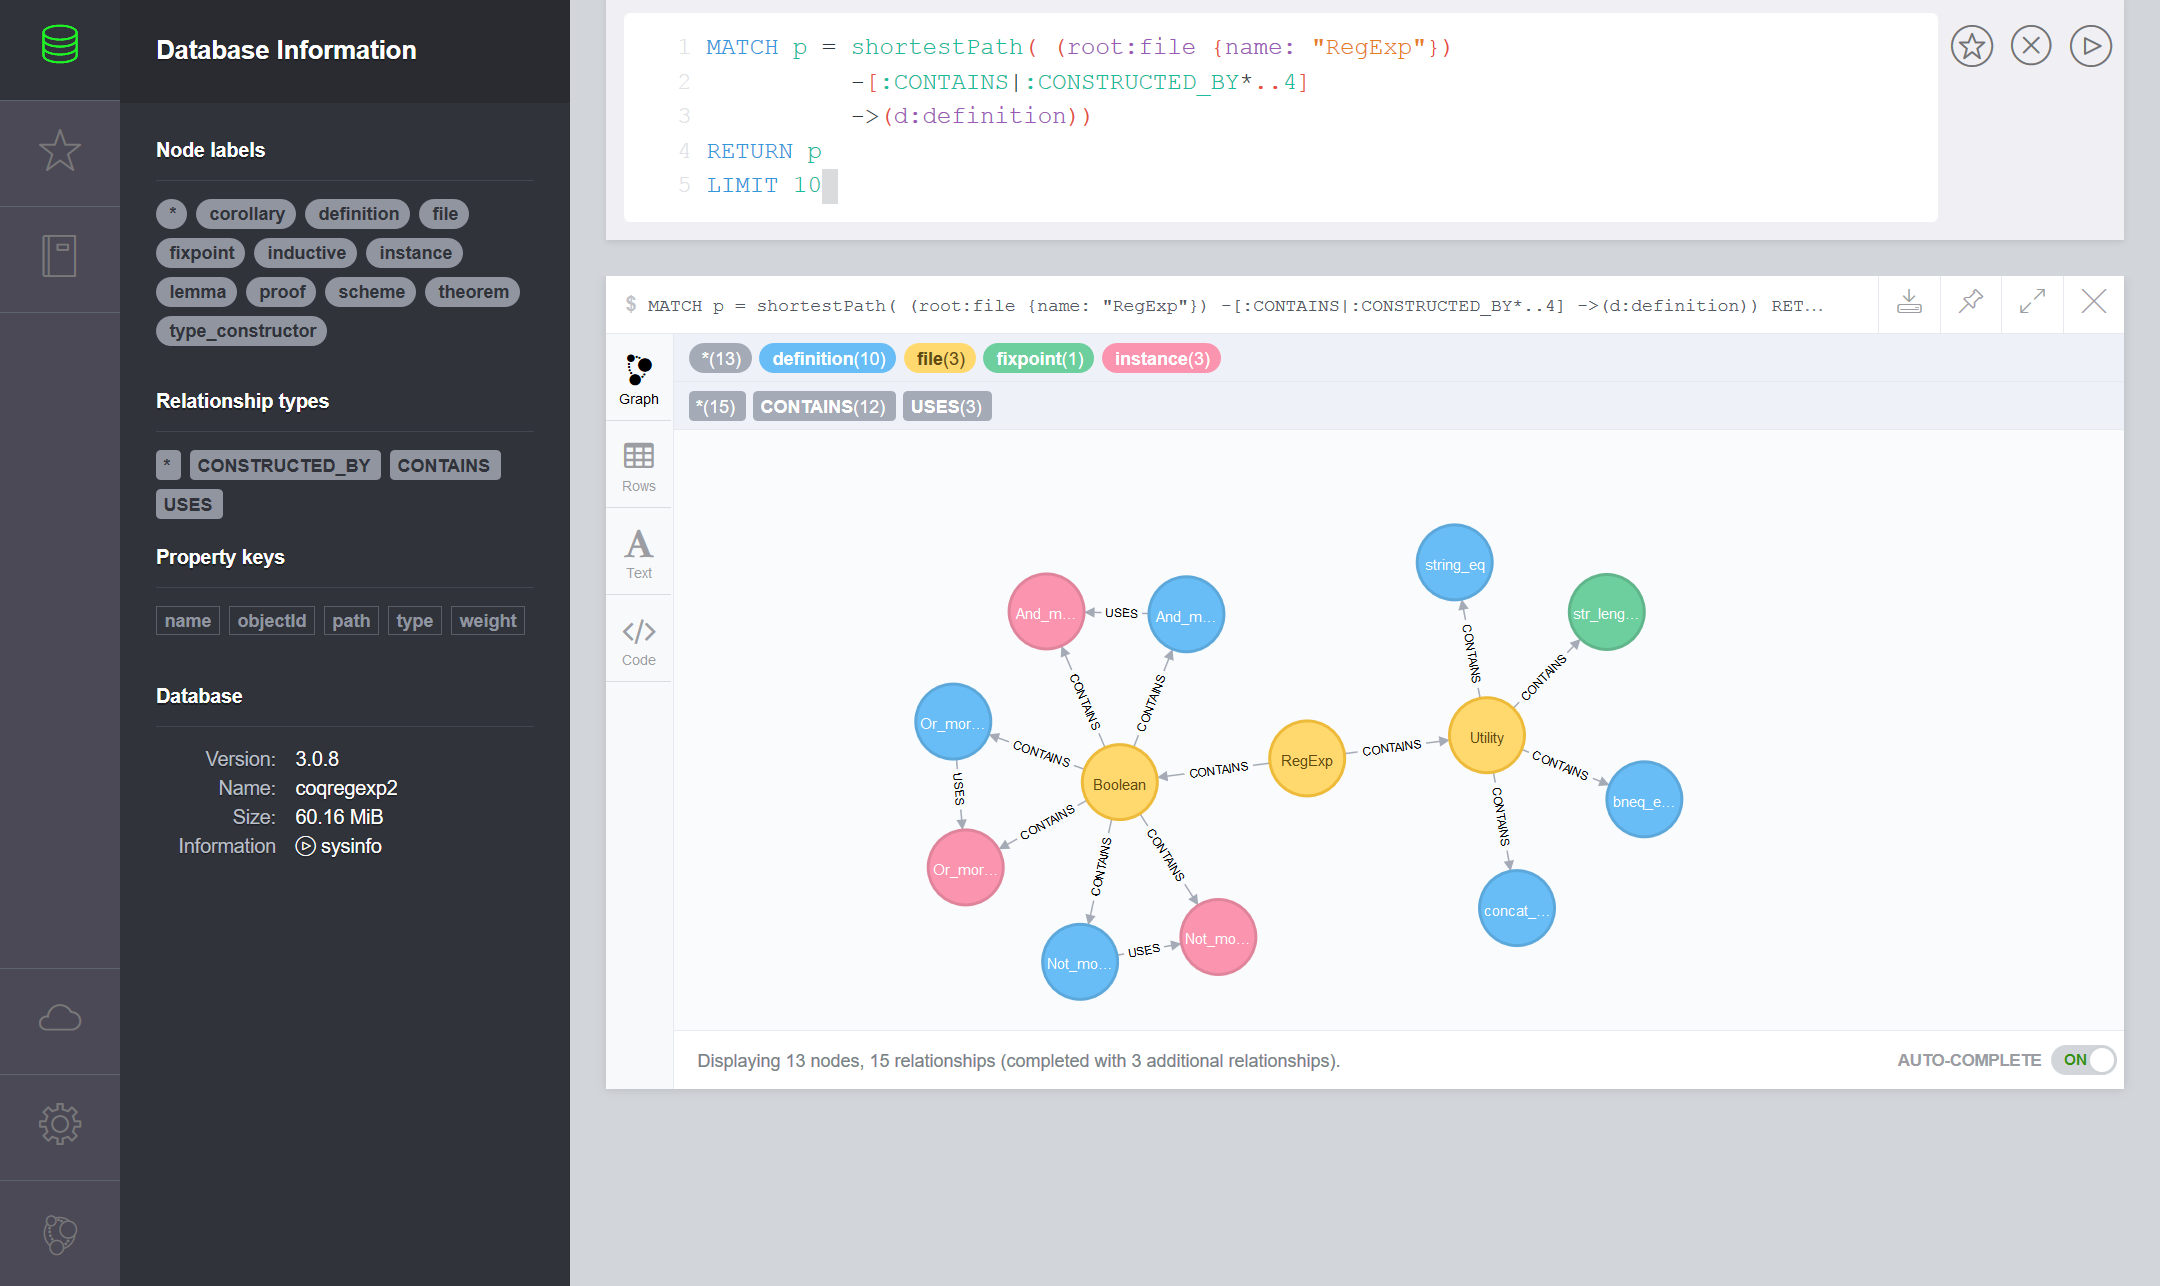
\includegraphics[width=\textwidth]{img/Neo4j_Browser.png}
  \caption{Neo4j Interactive Browser}
  \label{fig:neo4jbrowser}
\end{figure}

\subsection{Existing Tools for Neo4j}

\subsubsection{APOC: Awesome Procedures on Cypher}

\href{http://github.com/neo4j-contrib/neo4j-apoc-procedures}{\emph{Awesome
Procedures on Cypher}, or \emph{APOC}} for short, is a community-maintained Java
plugin featuring several graph algorithms callable from within Cypher itself.
Although there are other extension libraries (such as MazeRunner), APOC is well
documented, up-to-date and the most comprehensive, and therefore the obvious
choice as a foundation. By being a Java library hooked into Cypher, it offered
the potential for additional functionality to be built on top of it which
packaged-up some of the more complex features into \emph{domain-specific}
queries, intended for Coq users not familiar with Neo4j to get started with.
Thus, APOC helps step towards meeting the \emph{interaction} requirements for
this project by being easy to understand, flexibile to use and extensible; even
going part-way towards meeting the \emph{computation} requirements.

\subsubsection{igraph}

APOC has some key strengths that made it a good choice: it is easy to install
and use and has some basic graph algorithms to get started with.  However, its
main focus is on interacting with and combining different sorts and sources of
data and so lacks graph analysis functionality \emph{beyond} the basics. The
fact that it is implemented in Java further adds to its limitations: it is not
well-suited to more intense analyses over large graphs of libaries and is
insufficient to \emph{fully} meet the \emph{computation} requirements of this
project.

For such tasks, \href{http://www.igraph.org}{igraph} is ideal: it is described
on its website as a \emph{collection of network analysis tools, with the
emphasis on efficiency, portability and ease of use}. Written in C/C++ (with
bindings for R and Python), igraph offers a \emph{comprehensive} set of graph
algorithms without sacrificing on performance. These alogrithms and their uses
will be described later, in the Implementation chapter. For now, it suffices to
surmise that although igraph is not as easy to interact with (via the
statistics-oriented programming language R, as detailed in the next paragraph)
as APOC, the extra capabilities afforded were indispensible towards achieving
the \emph{computation} requirements of a core library of good defaults.

\subsubsection{visNetwork}

With igraph and APOC providing starting points for the computational aspects of
the projects, and the interactive Neo4j browser providing a well-polished,
graphical mode of interaction with basic, but useful, visualisation, the last
piece of the project was to incorporate the extra information gained from
\emph{executing} the graph algorithms.

\emph{Several} visualisation programs exist for Neo4j; however, many are for
commercial, industrial use and offer the features/complexity (and pricing) to
match. All tools which offer live visualisation with built-in Cypher query
execution (e.g. KeyLines, TomSawyer, Linkurious) are proprietary, requiring a
fee to use and offering more granularity than required. Offline (and
open-source) solutions (which require data to be exported in some manner before
visualisation) such as Gephi or Alchemy.js offer similarly many features, but at
the cost of a steep learning curve.  Ultimately,
\href{http://datastorm-open.github.io/visNetwork}{visNetwork}, (an R library
exporting to JavaScript which can be rendered inside a browser) was chosen due
to its simplicity and ease of integration with previous tools mentioned above.

\subsubsection{R}

\href{http://www.r-project.org}{R is a statistics-oriented programming language},
part of the Free Software Foundation's GNU poject. It is relevant for this
project because it offers an easy way to tie together Neo4j (through official
bindings), igraph and visualisation using visNetwork. This convenience came at
the price for having to learn R for this project, having been unfamiliar with it
prior. Nonetheless, it is a well-documented, relatively easy to pick-up language
and offered even more opportunities for learning during the course of this
project.

\section{Summary}

A detailed account into the planning of this project was given. The choice of
development methodology (spiral) and development tools (Git, GitHub, Travis-CI)
were noted. Requirements on modelling, interaction and computation were
explained and the choice of technologies and tools used as statrting points
(Coq, OCaml, dpdgraph, Neo4j, APOC, igraph, R and visNetwork) were justified
\emph{in relation} to \emph{which} requirements they satisfied.
